\documentclass[12pt,a4paper]{article}
\usepackage{times}
\usepackage{durhampaper}
\usepackage{harvard}
\usepackage{graphicx}
\usepackage{longtable}
\usepackage{siunitx}

\citationmode{abbr}
\bibliographystyle{agsm}

\title{Enigma and BOMBE Simulation}
\author{A.L. Gillies}
\student{A.L. Gillies}
\supervisor{M. Johnson}
\degree{MEng Computer Science}

\date{}
\begin{document}
\maketitle

\begin{abstract}\\

{\bf Context/Background} - The Enigma and BOMBE formed the basis of communication throughout the Axis powers. Technology has advanced since then, but how much? This will be the foundation of this paper, how much faster are we now, than then?\\

{\bf Aims} - Using the known execution speed of the antique Enigma and BOMBE, the aim of this paper is to show, through implementation and testing of a modern interpretation of the Enigma and BOMBE, the magnitude of speed up that has occurred since the inception of both.\\

{\bf Method} - Both machines have been re-created using modern technology and techniques, they have been timed, and this measurement will be compared to the same measurement on the original machine.\\

{\bf Results} - The modern versions of both are far faster than their antiquated counterparts. The magnitude of which can be seen in the results section.\\ Needs more \\

{\bf Conclusions} - The significant leaps that have been made in computing in the last 70 years cannot be overstated, The development from electro-mechanical devices to the silicon based computers we have today are astounding.
\end{abstract}

\begin{keywords}
Enigma, BOMBE, Parallel, Modern, Computation, Evaluation, Reinterpretation, Comparison, C++, Antiquated.
\end{keywords}



\section{Introduction}

\iffalse
What the project is about - talk through the motivations and a rough outline of the project\\
The project aims to show that a significant speed up has occurred in the field of computation since the inception of this cryptographic technique.
Context of the project - what are some real world things that need to be taken into account\\
What was achieved - go through deliverables and then go through issues and counter\\
2-3 pages\\
\fi

Since the time of Alan Turing, the developments of computational power cannot be understated. We have developed from electromechanical devices that have a single function, to electronic devices that are capable of renders and simulations of electromechanical devices within themselves, the BOMBE is an example of an electromechanical device and this can be rendered and simulated within a modern mobile device, let alone the cutting edge, which at the time, the BOMBE was. Within more cutting edge technology we are able to study models of the universe, and other academic pursuits that were inconceivable at the time of Alan Turing.\\

Alan Turing is the man that is credited with the creation of the BOMBE, this electromechanical device is then credited with breaking the German Enigma codes that are encrypted using the Enigma machine, this is another electromechanical device with a single function, it is used to encrypt messages that are then sent to another enigma machine that will then encrypt the message. This is how almost all of the German orders were relayed. The breaking of this code is said to have shortened the second world war by several years and thus save innumerable lives.\\

The motivations of this project are two fold, the first is to show the effectiveness of both the Enigma machine and the BOMBE. This will be done via the implementation of both in a modern setting. The second is to outline the developments that have occurred since the inception of the Enigma and BOMBE, by showing the significant increase in computational efficiency, an analogue for this would be how fast the BOMBE breaks the Enigma code. The most simple solution will be a BOMBE representation using modern coding techniques without any parallel improvement or any other modern techniques. This will be purely a copy of the enigma, in C++ code. This will outline the improvements between an electromechanical device and the sequential electronic devices that have been common from around the 1980s. The second, more complex solution will incorporate parallel programming, this was introduced in the early 21st century, and is still an improving technology.\\

\subsection{Deliverables}

\label{units}
\begin{longtable}{ |p{1.25cm}|p{4cm}|p{7cm}| }\hline\hline
Unique ID & Deliverable & Description \\ \hline
DL1 & Simulate the Enigma Machine & Have a working Enigma machine that can take in settings and plaintext and return ciphertext. \\ \hline
DL2 & Simulate the Bombe & A working BOMBE that takes in settings and ciphertext and returns decoded plaintext. \\ \hline
DL3 & Show the correctness of the Enigma Machine & Show through a series of tests and validations that the plaintext fed to the Enigma Machine and the Ciphertext returned are paired through the settings of the enigma \\ \hline
DL4 & Show the correctness of the BOMBE & Show that the known plaintext of the ciphertext input into the BOMBE is exactly the same as the plaintext that is returned by the BOMBE \\ \hline
DL5 & Evaluate average computation time over set inputs for both Enigma and BOMBE & Using a wide range of known plaintext - ciphertext pairs find the average computation time, the time take on average to do a single encode or decode for both simulations \\ \hline
DL6 & Parallelise The BOMBE and evaluate average computation time & Using known parallelisation techniques increase the speed at which the BOMBE will decode a given ciphertext \\ \hline
\end{longtable}

\section{Related Work}

\iffalse
Survey relevant literature\\
Relate to your own project\\
This should contain all details of the OG BOMBE and Enigma\\
May be able to reuse parts of the literature survey\\
use anything relating to parallel computing, the introduction of common single core computing, the introduction of C++ code, the development of the intel tool set, any historical papers about the enigma code, anything about the BOMBE, anything about the measurement of computational improvements.\\
2 pages\\
\fi

The electromechanical device known as the Enigma machine is best known for its use by the Third Reich, it was first designed by a company called Scherbius \& Ritter in 1918, and then sold to the German armed forces, after a few incremental upgrades. The machine is designed to allow secure cryptographic messages between two of these machines, the first will encode the message using decided settings, the second will, using the same setting, decode the message. This is done through a set of alphabet mapping, a one to one relationship between one alphabet and another, one letter is mapped to another and this relationship is bidirectional. No two letters from one alphabet map to the same letter in another.\\

The Enigma machine is made up of 7 parts, there are only 5 important parts plus an additional component and some wiring to make it work. The important parts are the plug-board, the three rotors, and the reflector. The other parts are a converter that allows all the separate components to work together, along with a lamp-board to show the encrypted letter, along with wiring to connect them all together.\\

The plug-board is a mapping from one alphabet to another that is a manual process of re-plugging 26 wires that map from one to the other. This does not change for each letter that is input into the device, unlike some of the components we will see later. The reflector is much the same as the plug-board, except that it cannot map a letter to itself. It is a simple one to one mapping that does not change over time, in the earlier designs of the Enigma machine, it could not be rewired, and instead had to be swapped out for another reflector with different wiring, in a similar way to that of the rotors that we discus later on, with later designs came the ability to rewire it. The rotors are the core of the machine. These are three modular, circular, mappings that are altered each time a letter is encrypted by the machine. The way they work is that the inner ring and outer ring each have contacts on them, when the outer ring is rotated then the mapping will change. there are 26 different mappings that can be used. The three rotors are chosen from a set of available rotors and each one has a unique ordering of letters on both its rings. Thus the order in which the rotors are input into the machine is important.\\

The enigma machine will take the first letter of the message that is to be encrypted from a keyboard and first pass it through the plug-board, it will then go to a converter which allows the signal to be passed to the first rotor, another mapping, then the second, and the third, in each of these case the inner ring of the previous rotor is connected to the outer ring of the next rotor. Then the reflector is reached, the mapped letter is then passed to the inner ring of the third rotor and this is a reverse mapping. The outer ring of the third rotor is connected to the inner ring of the second rotor and thus the signal will pass back through the rotors in this fashion. Once the plug-board is reached, the reverse mapping is done and a light will trigger on the lamp-board showing the letter that the input letter has been mapped to. After this the rotors are then stepped, this means that the first rotor will rotate one position for each letter that is encrypted. The second rotor will only step when specific notches are reached on the first rotor, the third is the same but for notches on the second rotor. Based on this method the first rotor will rotate more than the second and the second will rotate more than the third.\\

The BOMBE developed at Beletchly Park was very similar to the Enigma, but its antithesis. The BOMBE was based on a probably phrase attack, this means that for the BOMBE to work there needs to exist a known or guessed portion of ciphertext and its corresponding plaintext. An example of this that was used regularly was the German equivalent of "Weather Report", this was done daily and could easily be guessed. Once this was established then the exact letter to letter transformation must be established, this is done through the matching of letter to letter in the phrase such that no letter is encoded as itself as this is impossible for the enigma. Examples of these matching shown in figure one.

\begin{figure}[h]
\centering
Figure One
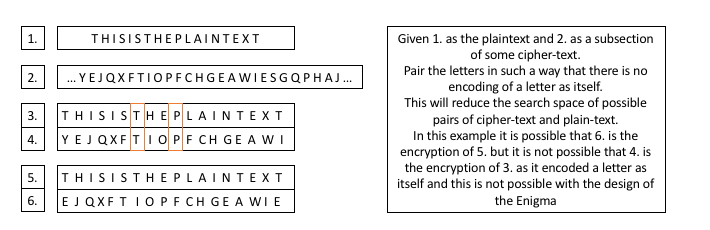
\includegraphics[width=\textwidth]{StageOneBOMBE.png}
\end{figure}

The next stage of preprocessing is the creation of crib-ciphertext pairings. This is the mapping of a specific letter at a specific set up of the enigma. For example in the figure above we can see that T maps to E at the first set up of the Enigma, at the second set up of the Enigma, because due to the rotor stepping we are now in a different set up, H maps to J, and so on. These pairs can then be joined to create a graph of pairings with the numbered setting as a label for the edge, a random example is shown in figure two.

\begin{figure}[h]
\centering
Figure Two
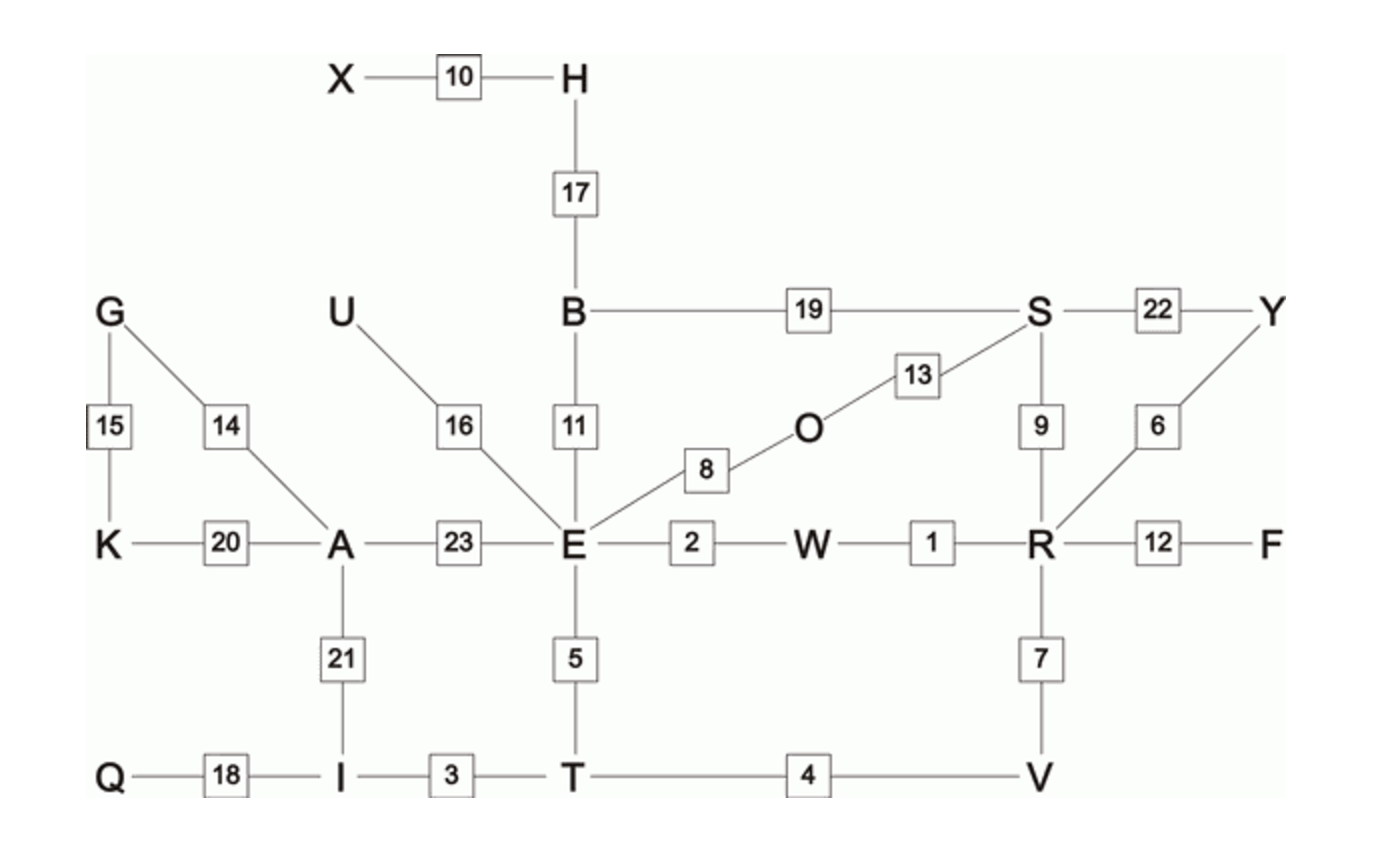
\includegraphics[width=\textwidth]{StageTwoBOMBE.png}
\end{figure}

There are significant implications that can be drawn from the connection network, the graph of pairings in figure two. Using the connection network the search space can be reduced by using the implications of some transformations on others. We first must recall that each transformation consists of two 'stecker swappings' and a 'scrambler encryption' these are the set of rotor transformation and reflector respectively. A 'stecker swapping' is the transformation of a letter through use of the three rotors that are present in the enigma, a 'scrambler encryption' is the transformation via the reflector, and then another 'stecker swapping' is the use of the reverse direction of the rotors. A relative position is the numbered set up that the enigma is currently in, so the first letter input into the enigma machine is using relative position 1, which is simply a set up of the enigma, relative position two is the set up of the enigma given that a letter has already been input and that the set up has changed due to the way the rotors behave. Using the connection network above, here is an example of the search space reduction that can be done using these details.\\

For example, let us test the hypothesis that E is mapped to K through the first three rotors, also known as E is "steckered" to K. Now consider how E is transformed into A at relative position 23, this is shown on the connection network above.

If E is "steckered" to K, K will be input to the reflector or "scrambler" at relative position 23 which will output some other letter L1. Since we know that E transforms into A at relative position 23, we know that A must be "steckered" to L1.

But if A is "steckered" to L1, L1 will be input to the "scrambler" at relative position 21 which will output some other letter L2. Since we know that A transforms into I at relative position 21, we know that I must be "steckered" to L2.

But if I is "steckered" to L2, L2 will be input to the "scrambler" at relative position 3 which will output some other letter L3. Since we know that I transforms into T at relative position 3, we know that T must be "steckered" to L3.

But if T is "steckered" to L3, L3 will be input to the "scrambler" at relative position 5.

Now consider the output of the "scrambler" at relative position 5 when it receives L3 as its input. Since we know that T transforms into E at relative position 5, we know that the output letter of the "scrambler" at relative position 5 must be "steckered" to E.

Suppose, when given L3 as its input, the "scrambler" at relative position 5 outputs J. By our original hypothesis E is "steckered" to K, but by our chain of implications E is "steckered" to J, so in this case E is "steckered" to both K and J. But the construction of the Enigma does not permit one letter to be "steckered" to two letters, so E cannot be "steckered" to both K and J, so our original hypothesis has resulted in an impossible consequence and so must be false.

But now suppose, when given L3 as its input, the "scrambler" at relative position 5 outputs K. Then by our original hypothesis E is "steckered" to K, and by our chain of implications E is "steckered" to K, so in this case E is "steckered" only to K, thus our original hypothesis has resulted in a consistent consequence and so may be true.

The altered connection network bellow shows the hypothesis that E is "steckered" to K via the the steps of implication that we have been through.

This is the way that the preprocessing that was done helped reduced the search space that it would have to be iterated through by the BOMBE and thus reducing the time taken for a result to be found.

The way the electro-mechanical device was created is very similar to an exploded view of the Enigma, it was created so that there would be no return journey through the rotors, instead another three rotors were added after the reflector. They were added in such a way that one pass through these 7 components is the equivalent of a pass through to the reflector and back through the rotors of the Enigma. The BOMBE was made up of three batteries of 12 sets of these 7 components. With the use of a "menu", also known as the connection network, this monstrous machine could be wired up so as to eliminate as many combinations as possible.\\

The next stage of the BOMBE set up is the plugging-up of the BOMBE. This is done with the help of what is known as a diagonal board, this was created by Gordon Welchman, as it encapsulated the reciprocal property of the Enigma, meaning that if R was steckered to Q then Q was steckered to R and so on for every pair in a specific Enigma set up, this could be used to eliminate parts of the search space. The diagonal board was used in conjunction with the menu or connection network to plug-up the BOMBE. The diagonal board consisted of 26 cables each containing 26 wires leading into and out of it, with a total of 325 connections between them. For example, the a wire in the B cable was permanently connected to the b wire in the A cable, and the a wire in the C cable was permanently connected to the c wire in the A cable, and so on. The effect of the diagonal board, when attached to the bombe, was to increase the feedback into the double-ended scramblers and thus reduce the necessity of obtaining loops in the crib-ciphertext pairing. This in turn made it possible to use shorter menus which were less likely to include a turnover of the Enigma's middle rotor during the encipherment of the plaintext. This is highly advantageous for reasons that will appear later. Once we have a menu and the diagonal board it will be plugged up such that, each rotor bridges two of the diagonal boards cables, when all the rotors have been connected in this way they are rotated to the positions in accordance to the relative positions in the menu. Next we mount the drums on their shafts. We first select a particular rotor order to try. Suppose we try rotors one, two, and three. We mount nine rotors each of which corresponds to rotor number one on the first nine top shafts in a battery, then we mount nine rotors each of which corresponds to rotor number two on the first nine middle shafts in the same battery, then we mount nine rotors each of which corresponds to rotor number three on the first nine lower shafts in the same battery. The other two batteries are now plugged up in exactly the same way except that different drum orders are selected. Note that the loops in the menu are represented by loops in the plugged-up bombe.\\

We will go through a simplified example of this using an eight letter alphabet, as using twenty six would be overwhelming. We will use the first eight letter of the alphabet, and the principles will be identical to that of the twenty six alphabet version of the BOMBE.

\label{Crib and Ciphertext}
\begin{longtable}{ |p{1.25cm}|p{1.25cm}|p{1.25cm}|p{1.25cm}|p{1.25cm}|p{1.25cm}|p{1.25cm}|p{1.25cm}|p{1.25cm}| }\hline
1 & 2 & 3 & 4 & 5 & 6 & 7 & 8 & 9 \\ \hline\hline
B & E & A & C & H & H & E & A & D \\ \hline
E & D & B & G & E & A & H & D & B \\ \hline
\end{longtable}

\begin{figure}[h]
\centering
Figure Three: 
From this table we can derive the menu or connection network.
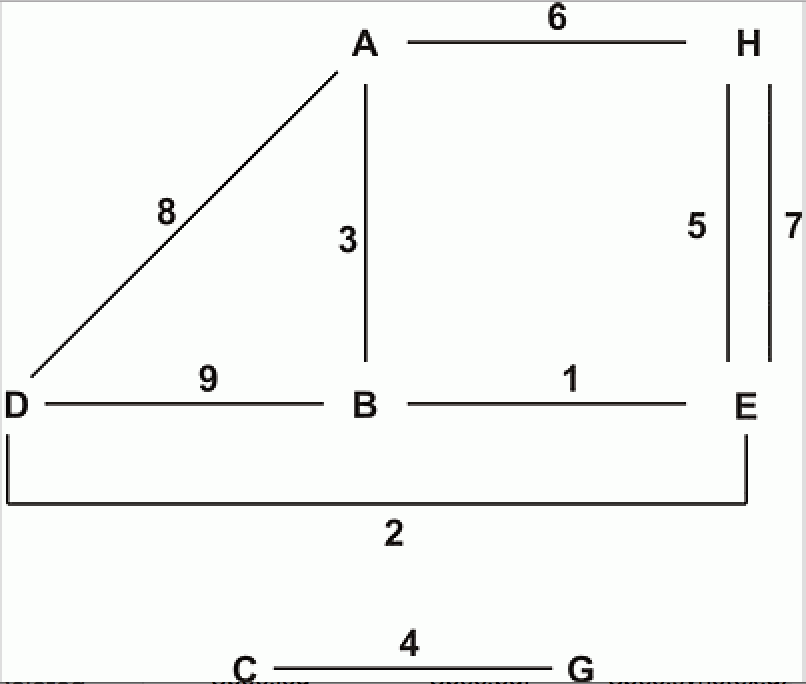
\includegraphics[width=0.5\textwidth]{BOMBEone.png}
\end{figure}

\begin{figure}[h]
\centering
Figure Four: 
This is the equivalent diagonal board for an 8 letter alphabet.
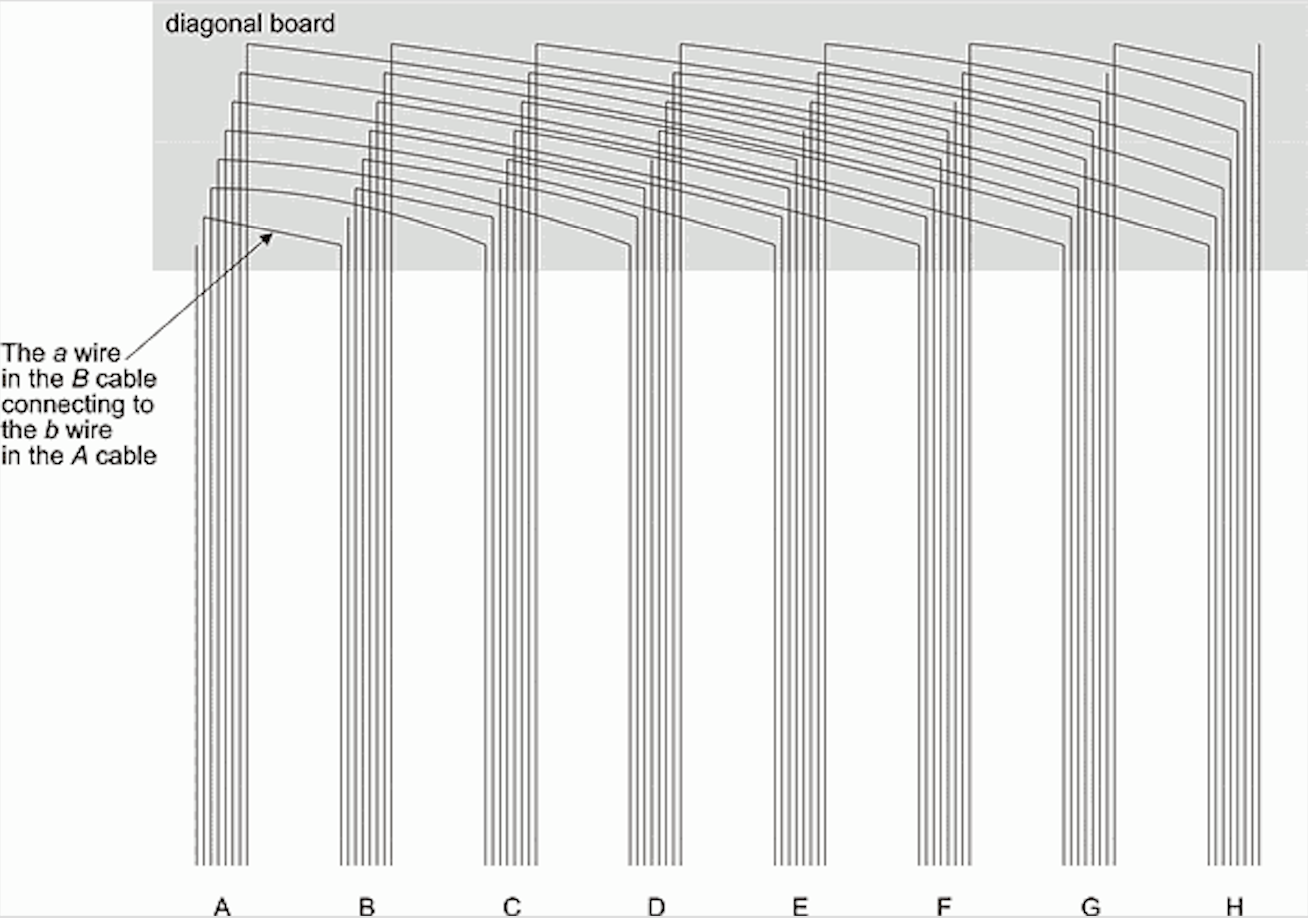
\includegraphics[width=\textwidth]{BOMBEtwo.png}
\end{figure}

\begin{figure}[h]
\centering
Figure Five: 
This is the fully plugged up diagram of an eight letter BOMBE.
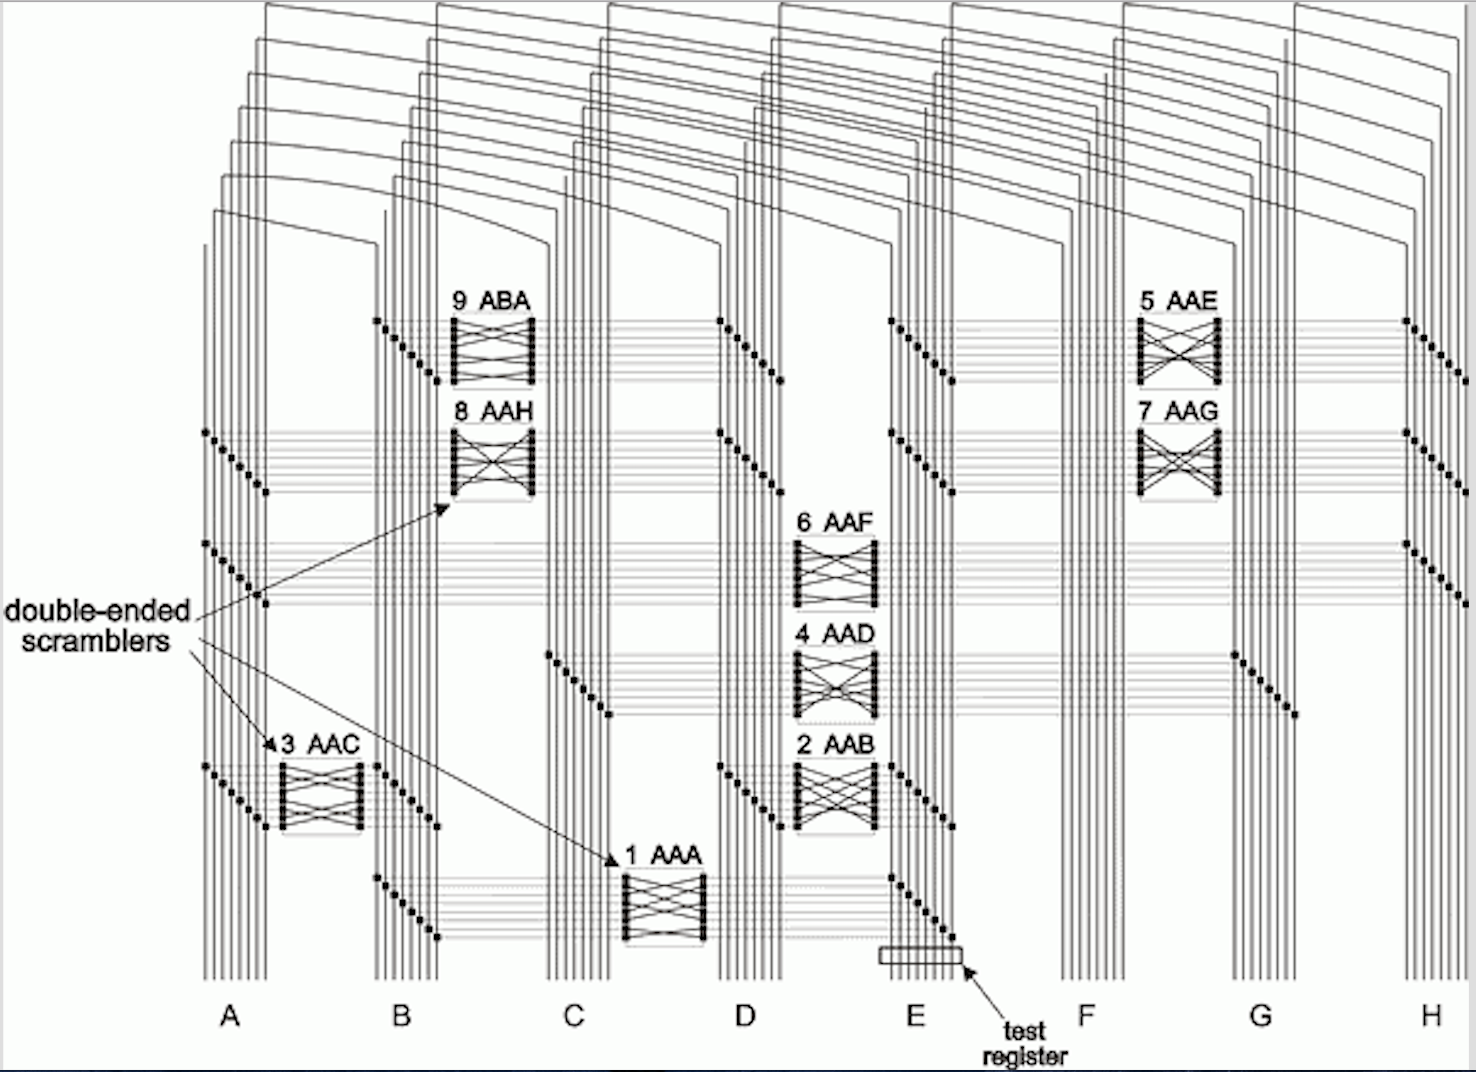
\includegraphics[width=\textwidth]{BOMBEthree.png}
\end{figure}

Once the BOMBE has been plugged up, it will be set in motion, this consists of the top row row of rotors stepping at a rate of 120rpm, with the second row of rotors at 1/26th that, then the third row at 1/26th that. They will continue to step until a "Stop" is reached or the rotors return to their original position. A "Stop" is defined as the transformations defined by the settings used yield the ciphertext from the crib. This was known by the BOMBE due to the test register. This was attached to one of the cables of the diagonal board, the 26 wires in a cable pass through the test register, with the test register being able to tell how many of its wires were "live" at any given time. When the bombe was started it applied a voltage to an arbitrary wire in the test register's cable, say the a wire in the E cable, to represent the hypothesis that A is steckered to E and E is steckered to A. Every wire connected to the a wire in the E cable and the e wire in the A cable would immediately become live, but suppose that another wire in the E cable, for example the h wire, becomes live. This represents the hypothesis that H is steckered to E and E is steckered to H. But E cannot be steckered to both A and H so we have arrived at a contradiction and we know that this rotor order, with this rotor position and the hypothesis that A is steckered to E is false. Having applied the current to the a wire in the E cable and therefore the e wire in the A cable and having had the current return to the h wire in the E cable and therefore the e wire in the H cable, we note that the current will pass through any scrambler connected to the A, E and H cables to wires in other cables which will not generally be the wires already energised in the A, E and H cables. Thus as the current flashes through the cryptanalytical circuitry of the bombe feeding back into cables and scramblers, more and more wires become live until, with a good menu, the feedback will almost always make all the wires in the test register live. There are two notable exceptions.

Suppose that the rotors are in the correct position but that the hypothesis being tested is false.
For example, suppose that the rotor order and position is correct and that the false hypothesis that E is steckered to A is being tested. This situation is shown in Figure 4.1 in which the thick black lines indicate those wires which are live after a voltage has been applied to the a wire in the E cable. In this case the wires representing the true hypotheses are not connected to the wires representing the false hypotheses. But, for the reason discussed above, the wires representing the false hypotheses are connected together so when any one of them has a voltage applied to it, the voltage appears on all of them. So, in this case, if we look in the test register we will find exactly 25 live wires and one dead wire. The dead wire, and all the wires connected to it, indicate stecker swapping consistent with the crib-ciphertext pairing. See figure six.

\begin{figure}[h]
\centering
Figure Six: The bold wires indicate a "live" wire. The dead wires in the cables indicate that A is steckered to G, B is steckered to E, C is self-steckered, D is steckered to F, and H is self-steckered.
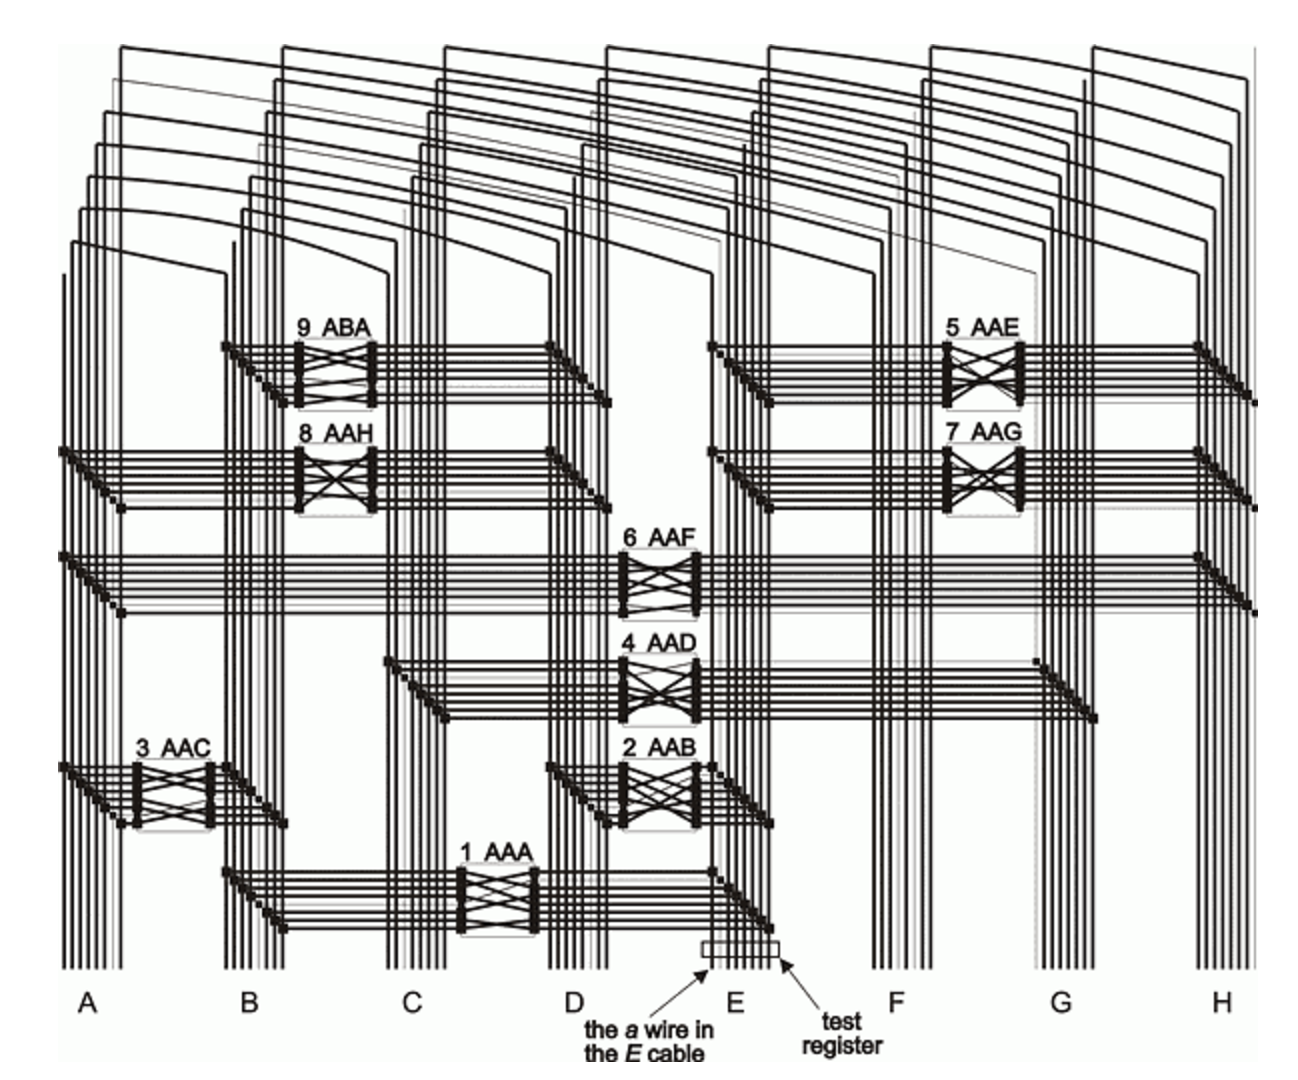
\includegraphics[width=\textwidth]{BOMBEfour.png}
\end{figure}

Now suppose that the rotors are in the correct position and that the hypothesis being tested is true. For example, suppose that the rotor order and position is correct and that the true hypothesis that E is steckered to B is being tested. This situation is shown in figure seven, which has exactly the same scrambler positions as figure six and in which the thick black lines again indicate those wires which are live, this time after a voltage has been applied to the b wire in the E cable. In this case the wires representing the true hypotheses are not connected to the wires representing the false hypotheses so when a voltage is applied to any one of the wires representing a true hypothesis, the voltage appears on all the other wires which also represent true hypotheses, and on no other wires. So, in this case, if we look in the test register we will find exactly 1 live wire and 25 dead wires. The live wire, and all the wires connected to it indicates stecker swapping consistent with the crib-ciphertext pairing. In the example shown in figure seven, the live wires in the cables indicate that A is steckered to G, B is steckered to E, C is self-steckered, D is steckered to F, and H is self-steckered, in other words, the steckering that the bombe has found is identical to that of figure seven. The wires which are live in the test register in these two situations are the logical complement of each other. So there are two stop conditions which the bombe looks for, either exactly one live wire or exactly 25 live wires in the test register.

\begin{figure}[h]
\centering
Figure Seven
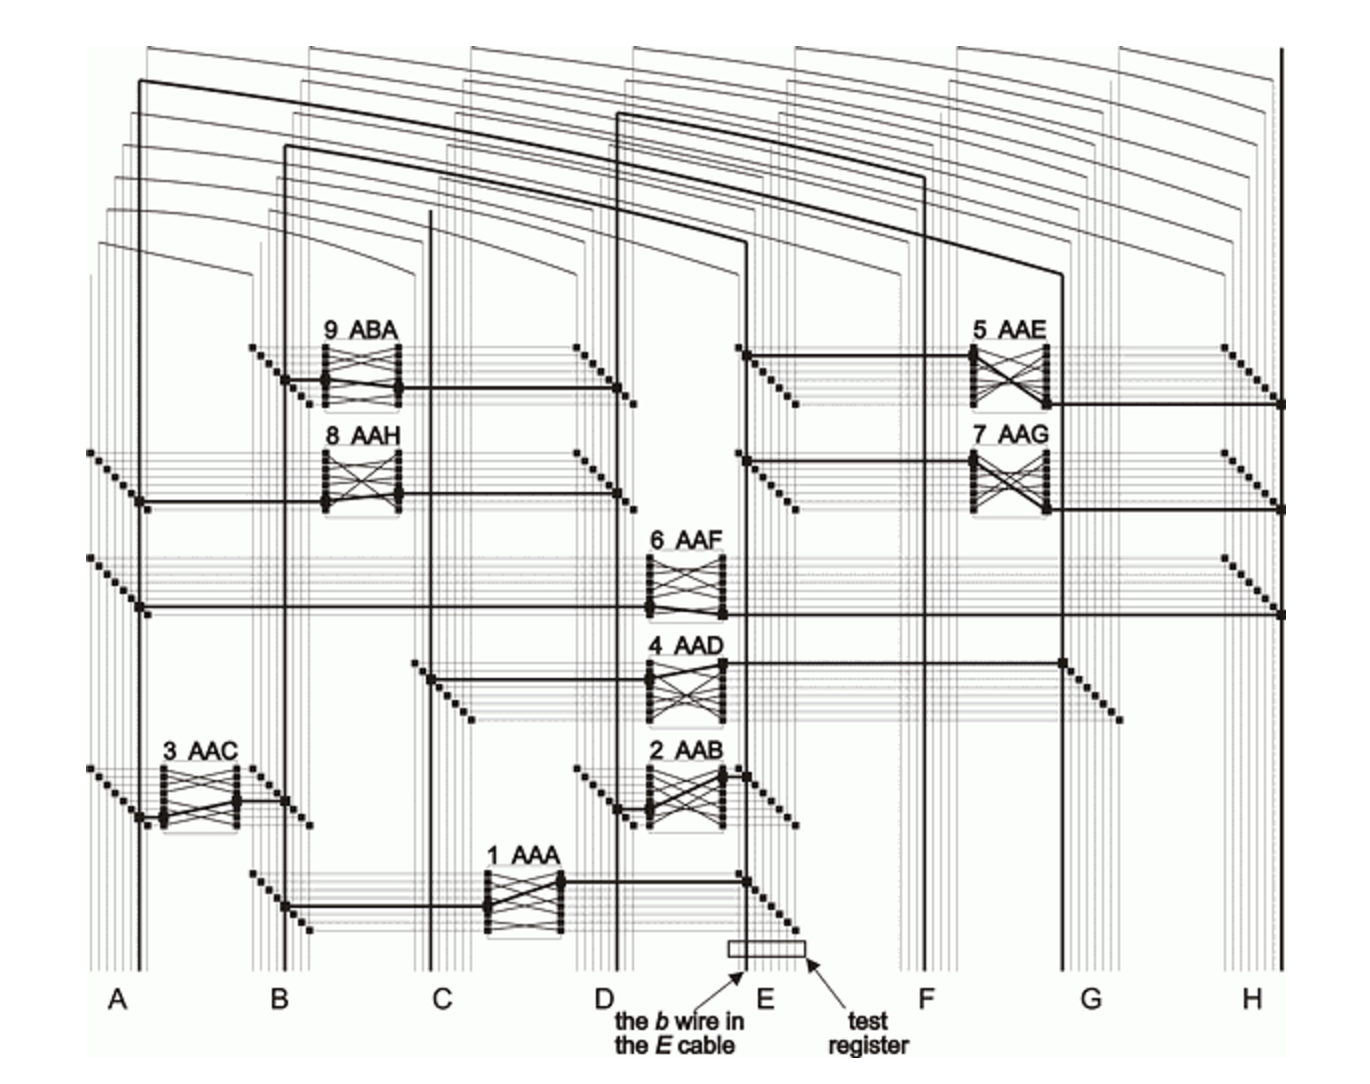
\includegraphics[width=\textwidth]{BOMBEfive.png}
\end{figure}

Once a stop had been established, it would then be tested. This was a manual process, usually done by one of the operators of the machines known as wrens. The question may now be asked, "What about the plug-board?", this was still done manually, and only done after a stop had been found. The breaking of the plug-board is straightforward enough, due to the fact it does not change as the letters are input, so if the setting detected by the stop are correct then this can be broken by frequency analysis. Frequency analysis is the process of matching frequency of letter in the plaintext language and the letter frequency of the ciphertext language, for example, if in the ciphertext every other letter is an E meaning that half of all letters are an E, and in the corresponding ciphertext half of all the letters are Q then we can have an educated guess that E maps to Q. This is an extreme example, but the principle holds and can be applied to every letter in the alphabet used with the same process. This is how the plug-board is broken using the settings detected by the stop.

\section{Solution}

\iffalse
Overview of architecture and design - use parts from the design report\\
Description of tools used - design report\\
Outline of algorithms to be used - design report\\
Features of the implementation process - issues and struggles with the implementation, how they were overcome\\
Testing - validation and all other testing done\\
Verification and validation\\
Stages of the life cycle undertaken - software engineering\\
4-7 pages\\
\fi

\subsection{Enigma}

C++ was chosen as the implementation language for the enigma mainly due to its rich library, it has support for a wide range of external libraries, the main one we will be focused on in this case is the Intel tool set, this may not be much use when it comes to the Enigma but it is a very strong and well established tool that allows C or C++ code to be parallelised which is the aim of the BOMBE implementation that will be outlined later. The reason that C++ was chosen specifically for the Enigma implementation is that it is a middle level language and thus enables the benefits of low level and high level languages as well as being highly portable and non operating system specific. It is also very well established in the teaching at Durham University.\\

The recreation of the enigma machine was to be done in C++, this was chosen as it has significant parallel tools available for it, in the form of the Intel c++ compiler. A tool that has shown great capabilities in parallelism. This would be very helpful in the creation of the advanced BOMBE recreation and developing in two separate languages didn't make sense.\\

The recreation revolves around a settings file, this is a text file that contains all the setting that will be used by the enigma machine to encode the message that it is given through the command line interface, these settings include; the plug-board mapping, the reflector mapping, the rotors that will be used and their corresponding initial displacement. This file is then updated automatically to reflect the changes that have occurred to the settings as the message is encrypted, each letter will have a different set of setting as the displacement of the rotors changes, this will be reflected in the settings file. The c++ file that makes up the core of the code that has realised enigma, is called the main file, this will manage all the changes that occur as well as managing user interaction with the device and having a central location with which to manage the other c++ files that realise different parts of the enigma machine.\\

The plug-board, reflector, rotors, as well as a converter file have all been created in their own separate files so as to improve the modularity of the system, as well as provide a more focused development route; each file can be developed without removing functionality for the others.\\

The main file contains the instructions on how to use the system, it contains all file dependency instructions, as well as containing the set up function and main function. The set up function will be run before the system is usable, it will find the set up file, using the information that it contains, it will then make the system usable through the main function of the main file. As the set up function is run, it will call the set up functions of all the other parts of the enigma in other files, the plug-board file will store its mapping, the reflector will store its mapping and the rotors file will store the rotors that are currently in use and make sure that the displacement is correct for each one. Once this has been done the main function is used, this will take in user input through the command line, the only thing that will be input is the plaintext, this is the message to be encrypted. The main file will then iterate through each of the letter in the message and encrypt them individually, using unique settings for each letter. The first letter will use the settings that have been read in by the set up file. the first stage is to convert the letter to its corresponding number, for example A is equal to 1 and Z is equal to 26, this makes use of the converter file, this file contains functions to convert between letters and numbers as well as another function that does the reverse. This was done because numbers are much more manageable than letters in terms of computation. once this has been done the number will be sent to the plug-board. The plug-board stores the mapping from one set of 26 numbers to another set of 26 numbers, this is a computational realisation of the alphabet to alphabet mapping that is done by the electromechanical enigma device. Once this has been done in the require direction, the plug-board has two directions mapping forwards and mapping back, we will use the mapping forward function now, and the mapping back function at the end to receive the encrypted message. We have now finished the mapping through the plug-board and will move onto the first rotor. The first rotor will have been chosen by the user in the set up file as well as its initial displacement from its standard position. This is another alphabet to alphabet mapping, but with a twist. The twist is that each letter does not have the same mapping, once a letter has been encrypted the enigma machine will increment the displacement of the rotor and once the first rotor has reached a specific displacement it will increment the displacement of the second rotor which in turn may reach a specified displacement and cause the third rotor to increment its displacement. This is only done once the current letter has been fully encrypted, meaning once it has passed forwards through every rotor as well as back through them. Once the letter has been mapped by each of the rotors it reaches the reflector, this is very similar to the plug-board, it can be re-programmed in a very similar way. This mapping is then done, with the caveat that a letter cannot be encrypted as itself at this point, and the return journey begins. The letter will travel back through each of the rotors, this time being mapped in the opposite direction, then to the plug-board, which will also map in the backwards direction as mentioned before. This concludes the encryption of this letter, in the electromechanical enigma this would cause a letter to light up on the device to show which letter the input letter has been encrypted as, in this device, the covert file will be used, this is because throughout this process the 'letter' has actually been the number corresponding to that letter so as to simplify the process, we will map from number to letter and output this encrypted letter. Once we have a fully encrypted letter the rotors will change their displacement as the process will start again for the next letter in the message. This will continue for all letters in the message until we reach the end, at this point the new setting that the system is using will be output to the settings file, this is done so that we are not reusing the same setting each time we encrypt something as the set up function will be reading in the same values again and again from an unchanged settings file.\\

Once the Enigma was formed in its component parts, each was tested for expected behaviour. The plug-board was set up, and then each letter of the alphabet was input and the output validated, this was done multiple times with random settings as doing 26! tests was not feasible. The reflector was the next thing to be tested, this was done in the same way, each of the hardcoded reflectors are tested, then an identical test to the one performed on the plug-board is done, the reflector is reconfigured, and then tested, this is repeated until it is deemed that enough of the settings space has been covered. The rotors were also tested, there are eight rotors that can occupy any one of three positions, with no repetitions, and there are 17576 unique paths through any three rotors. This results in 984,256 possible unique routes through the rotors, with any three rotors chosen. Once all the individual components had been tested and passed their respective tests, the machine was set up in its entirety, meaning that we have a working enigma. A few preliminary tests were done to make sure that the enigma behaved as expected, these were known paths through the enigma done outside of the system manually, then shown to behave the same within the system.\\

The Enigma was built in pieces, firstly to make sure that each functioned as expected and could be tested independently of the others, and secondly that the development style would be able to avoid a waterfall model, where one thing is based on another and then another is based on that, this builds up a very significant reliance relationship between the components and thus causes significant issues if one of the first components to be created is found to have an issue further down the development chain. Instead of this method an agile method was adopted, each component developed individually, and simultaneously so as a foundation is established for each component then this is built upon until we reach the point that all components function as expected and they can then be used together in the final system. This circumvents the issue that a broken component results in more development time on a component that was reliant on the broken component, but was otherwise working as expected.

\subsection{BOMBE}

The main development tool for this project was the Intel toolset, this allowed testing of the hypothesis with the least overhead. This means that is a mature and well established tool that allows parallel techniques to be applied simply and with confidence. The reason that this tool specifically was used in conjunction with C++ was the reason that Fortran, the only other option with this specific tool, is seen by many as an antiquated language that is rather steep with its learning curve and with an already supposed high barrier for entry, this was passed over for the relatively easy to start and learn C++.\\

The first version of the BOMBE that was recreated in C++ code never actually existed, this was made as a benchmark for the others. In this version we will use a brute force approach with no limitations, that is we will try every combination of setting possible to attempted to map from the input encoded message and the guessed message that it corresponds to. This is done through a similar method to that which was used to make the Enigma Machine. In fact a copy of the exact enigma machine code was used in this implementation. The only difference is the main file and settings file, the main file will rewrite the settings file with each possible setting and then it will be tested, if the results are wrong then the next setting is used, this is done until the settings that were used in this case are found, they will then be output by the main file so that they might be used by an enigma clone to break any other messages that were sent in the same block as the message that was just broken and thus have almost identical settings. The brute force approach is slow. The reason that this approach is slow is that there are a lot of settings that have to be tested. Each of the components have their own complexity, and thus each have a number of settings that need to be iterated through. The plug-board, this has 26 letters in it, this means that there are 26! ways that this can be encoded, this does not change through usage however, this is a useful feature in the later BOMBE recreations but for this implementation, it is one of the more challenging components. The rotors, there are eight rotors that can be chosen to occupy any one of the three positions, this means that there are 56 different set ups that can be used from the eight rotors, each rotor then has 26 different displacements that can be used, meaning that total there is 17,576 different settings after three rotors have been chosen and 984,256 different set ups if any of the eight rotors can be chosen. The reflector has a very similar complexity of the plug-board however it cannot encode a letter as itself, meaning that there are 25! ways that it can be encoded. The results of this are that the brute force BOMBE has to go through \num{6.15705e57} different settings. The exact number of settings that need to be tested is actually; \num{6157051363093094576378463970354900547389095936000000000000}. This was known from the start, that is why it was done. This is the slowest that a BOMBE could possibly be using modern techniques. \\

The BOMBE recreation in C++ code was done in a very similar way to the Enigma, it is a main file that contains all the details and management, whilst other files contain the details and behaviours of the components that make up the BOMBE. The rotors and reflector as as they are in the Enigma, the files have not changed. The diagonal board is also an additional file that will be used to create the menu as well as test the BOMBE for stops. Once a stop has been found the details are input into a frequency analysis file that will then validate the stop is correct and then pass this information back to the main file, which will then output the correct settings. The only input that is needed by the main file is the ciphertext and guessed crib, this will then be passed to the diagonal board for a menu to be created, this is a function inside the diagonal board file. Once a menu has been made this will be passed to the diagonal board set up function, this will then create a computer model of what we see in figure five. This is the testing board for each of the settings output by the model of the enigma the is run from the main file. If a stop is detected, then these settings will be passed to the frequency analysis file, along with the crib and ciphertext, this will then run, and output the settings used in the plug-board, then all settings will be output by the main file. At this point we have the settings for all components that were used by the enigma to encrypt the ciphertext, any other messages sent in the same network as this message, which will use the same run of settings will be easily decrypted as the settings are already known.\\

The "parallelising" of the BOMBE was multistage, the first being the use of the brute force approach basis to allow for simple, single line commands for Multiple Instruction Multiple Dataset and Single Instruction Multiple Dataset techniques to be applied without anything more advance being used and the rest being left to the compiler. This resulted in a very substantial increase in performance, the Multiple Instruction Multiple Dataset technique split the workload across cores, this resulted in an almost N time performance increase from the non-parallel version. This is due to the lack of data dependencies and lack of overhead in setting up the file. The data that each of the cores was using was stored in the cache associated with each, the only thing that changed per core were the variables that store the settings currently being tested and the output that would be tested against the known ciphertext value, which was set to be immutable so that it could be treated as read only memory for each of the cores not resulting in any of the processes waiting for the use of the data. This was a very effective technique. The use of Single Instruction Multiple Dataset technique is less effective, this is the use of vectorised loads from memory, meaning that more than a single value can be retrieved from memory at a single time. This process is not significantly data dependant, most of the process is mostly reading data that cannot be vectorised, and even if it could be it would not be useful as the data load is specific to one letter from one data source then another letter from another data source, this continues until the next letter is input. This process, whilst having significant improvements from the original, the original takes such a long time that this approach is still slower than the time taken by the exact BOMBE recreation. The next stage of "parallelising" the BOMBE is the application of parallel techniques to the exact BOMBE recreation. This was based on the lessons learnt from the application of parallel techniques to the brute force BOMBE, that MIMD is much more effective than SIMD. This technique is applied to the settings search, by splitting the search space between all cores available means that there is an N times speed up, where N is the number of cores available. This means that there is still a fair amount of overhead, the frequency analysis cannot be sped up. The result of this is still a marked improvement.\\

The testing methodology is identical to that of the Enigma, each file was tested individually for consistency with expected behaviour, then joined to make the whole. The rotor and reflector file are identical to the ones used in the Enigma, they were previously tested. The diagonal board was tested through a incremental test, each of the 325 connections was tested for the expect "live" wires. Once this was done, the creation of the menu as tested. An exemplar ciphertext and crib were input and the result was tested against a manually made menu. This was done multiple times with different pairings. The behaviour whilst testing each of the rotors was also tested, but this required the BOMBE to be run from the main file as a whole, this was done at that stage. The frequency analysis was tested by taking multiple known examples and running them so make sure the result was correct, this is a deterministic process so the result isn't always perfect. This was a problem that was encountered in the original BOMBE as well. Once each of the components were tested, the BOMBE was built. This was then tested against random known encodings from the Enigma machine. The results were then compared to the plaintext and, due to the deterministic nature of the frequency analysis, a rough result was that one letter may differ in a 10 letter crib, this was considered enough to make out the word or message that was sent. If the message was of critical nature such that a single letter being wrong was going to cause an issue then the frequency analysis could be done manually as it was done originally, this was done once in the testing process to prove it could be done.\\

Again an agile approach was adopted for this project, each component is not dependant on another such that modularity and independent development was possible. This also allowed for independent testing, which was a key asset in the confirmation of the correctness of the BOMBE besides just the output being correct, it was shown to be correct throughout the process.

\section{Results}

Evaluation method description\\
Experimental settings - talk about the grid search done\\
Results generated by the software\\
2-3 pages

\section{Evaluation}

Discussion of strengths and weaknesses of solution and of lessons learnt - evaluate issues\\
Limitations of the solution - given more time... etc.\\
Critical appraisal of the way the project was organised - critique my own organization\\
2-3 pages

\section{Conclusion}

An overview of the project\\
Brief description of the main findings\\
Discussion on how the project can be extended\\
1-2 pages

\bibliography{REF}

\nocite{*}

\end{document}